\chapter{Desafios de Escalabilidade em Blockchain:Impactos }
\label{chapter_desafios_de_escalabilidade}

% Esta pesquisa tem como objetivo explorar os limites do Blockchain em relação à escalabilidade e capacidade de processamento de transações em grandes escalas, utilizando métodos sistemáticos de análise de literatura. O Blockchain, apesar de ser uma tecnologia revolucionária com grande potencial para transformar diversos setores, apresenta alguns desafios que podem afetar sua eficiência em larga escala.

% Um dos principais desafios do Blockchain é a escalabilidade, que se refere à capacidade da tecnologia de lidar com um grande número de transações em um curto período de tempo. Isso ocorre porque cada transação é validada por um grande número de nós na rede, o que pode resultar em um gargalo de processamento de dados. Além disso, a capacidade de armazenamento de dados também pode ser um desafio, especialmente em Blockchains públicos, onde todas as transações são armazenadas em cada nó da rede.


\section{escalabilidade}
Nesta seção, será discutida a escalabilidade do Blockchain, um aspecto crucial para o sucesso e adoção em larga escala desta tecnologia inovadora. A escalabilidade refere-se à capacidade da tecnologia Blockchain de lidar com um aumento significativo no número de transações e usuários sem comprometer sua eficiência e desempenho.

% A escalabilidade do Blockchain é um aspecto crucial para sucesso e adoção em larga escala do Blockchain. Refere-se à capacidade da tecnologia Blockchain de lidar com um aumento significativo no número de transações e usuários sem comprometer sua eficiência e desempenho.

Um dos principais desafios enfrentados em relação à escalabilidade do Blockchain é o tempo de processamento das transações. Cada nó da rede Blockchain precisa validar e registrar cada transação em todos os nós da rede, o que pode levar a atrasos à medida que o tamanho do Blockchain cresce. O mecanismo de consenso distribuído, como o algoritmo de prova de trabalho (Proof-of-Work), também pode exigir um tempo considerável para confirmar transações.

Além disso, o aumento do consumo de recursos computacionais é uma preocupação em termos de escalabilidade. Os nós da rede Blockchain, especialmente os nós completos que armazenam e validam todas as transações, requerem poder de processamento e capacidade de armazenamento significativos. À medida que o número de transações e a complexidade dos contratos inteligentes aumentam, a demanda por recursos computacionais também aumenta, o que pode levar a problemas de desempenho e custos adicionais. 

No contexto do Bitcoin, é crucial mencionar que existe um limite predefinido para o tamanho de cada bloco que comporta as transações. Isso implica que cada bloco é capaz de acomodar apenas um número limitado de transações. A visão inicial de Satoshi Nakamoto, o criador do Bitcoin, explicou em seu trabalho seminal \cite{Blockchain-Satochi} que a rede é projetada para adicionar uma média específica de novos blocos a cada hora.
Uma característica notável desse sistema é que, se a rede estiver processando mais blocos do que a média prevista, o desafio de Proof-of-Work se torna mais complexo. Esse ajuste dinâmico resulta no aumento da dificuldade do processo de mineração, o que, por sua vez, faz com que o número de blocos confirmados retorne à média desejada. Portanto, o ritmo de validação de blocos e, por extensão, o número de transações validadas, é limitado a cada hora.

É capital  observar que, à medida que a rede Bitcoin continua a se expandir, a capacidade de processamento de transações também enfrenta limitações. Este fato levou a situações, como observado em 2017, em que as transações de Bitcoin sofreram atrasos significativos, levando horas para serem confirmadas. Durante esses períodos de alta demanda, as taxas de transferência associadas a essas transações também aumentaram consideravelmente \cite{Guia_do_Bitcoin}.



\section{Capacidade de processamento de transacões em grande escala}

% Nesta seção, será abordada a capacidade de processamento de transações, um dos principais limites da tecnologia blockchain. Embora o blockchain seja projetado para ser um sistema descentralizado e seguro, sua arquitetura distribuída pode resultar em restrições em termos de velocidade e capacidade de processamento.

% A capacidade de processamento de transações é um dos principais limites da tecnologia do blockchain. Embora o blockchain seja projetado para ser um sistema descentralizado e seguro, a sua arquitetura distribuída pode resultar em restrições em termos de velocidade e capacidade de processamento.

% Um dos fatores que afeta a capacidade de processamento é o tempo de confirmação das transações. Em blockchains que usam algoritmos de consenso como Prova de Trabalho (Proof-of-Work), cada transação precisa ser validada e confirmada pelos nós da rede, o que pode levar algum tempo. Isso resulta em limitações na quantidade de transações que podem ser processadas em um determinado período.\cite{yang2019effective}

% Uma breve explicação do algoritmo de consenso Proof-of-Work (PoW), que, devido às suas características operacionais, pode tornar a rede do blockchain um pouco mais lenta.
Nesta seção, será abordada a capacidade de processamento de transações, um dos principais limites da tecnologia blockchain. Embora o blockchain seja projetado para ser um sistema descentralizado e seguro, sua arquitetura distribuída pode resultar em restrições em termos de velocidade e capacidade de processamento.

Um dos fatores que afeta a capacidade de processamento é o tempo de confirmação das transações. Em blockchains que utilizam algoritmos de consenso como Prova de Trabalho (Proof-of-Work), cada transação precisa ser validada e confirmada pelos nós da rede, o que pode demandar algum tempo. Isso resulta em limitações na quantidade de transações que podem ser processadas em um determinado período \cite{yang2019effective}.
Será apresentada também uma breve explicação do algoritmo de consenso Proof-of-Work (PoW), que, devido às suas características operacionais, pode tornar a rede do blockchain um pouco mais lenta.

\subparagraph{ \textbf{Prova de trabalho (Proof-of-Work)}}

O algoritmo de Prova de Trabalho (Proof-of-Work, PoW) é um dos mecanismos de consenso mais amplamente utilizados no contexto do Blockchain\cite{buterin2019next}. Foi introduzido originalmente por Nakamoto Satoshi no white paper do Bitcoin e tem sido adotado por várias outras criptomoedas e redes Blockchain \cite{Blockchain-Satochi}.

O objetivo do algoritmo de Prova de Trabalho é garantir a segurança e a integridade da rede, tornando computacionalmente custoso para um participante mal-intencionado atacar a rede ou modificar o histórico de transações. Ele exige que os mineradores resolvam problemas matemáticos complexos, conhecidos como "quebra-cabeças criptográficos" ou "hash puzzles", a fim de adicionar novos blocos ao Blockchain.\cite{yang2019effective}

Para resolver esses quebra-cabeças, os mineradores devem gastar uma quantidade significativa de poder computacional, que é medido em termos de poder de processamento (hashrate). O objetivo é encontrar um valor hash que atenda a certos critérios específicos, como ter um determinado número de zeros no início. Os mineradores tentam diferentes combinações até que um deles encontre a solução correta, e o bloco é adicionado ao Blockchain.

Uma vez que um minerador encontra a solução, ele a propaga para a rede, que então valida e aceita o novo bloco. O minerador que resolve o quebra-cabeça recebe uma recompensa em forma de criptomoeda, incentivando a participação no processo de mineração.

Embora o algoritmo de Prova de Trabalho seja eficaz em garantir a segurança do Blockchain, ele também tem algumas desvantagens significativas. Uma delas é o alto consumo de energia associado à mineração, especialmente em redes com um grande número de mineradores competindo por recompensas. Isso levou a críticas em relação à sustentabilidade ambiental do Bitcoin e de outras criptomoedas baseadas em PoW.

Além disso, o algoritmo de Prova de Trabalho pode resultar em um tempo de confirmação relativamente longo para as transações, uma vez que os mineradores precisam competir para resolver os quebra-cabeças. Isso pode limitar a escalabilidade da rede, especialmente em momentos de alta demanda por transações.
%%Outro desafio importante é a privacidade, já que o Blockchain é projetado para ser uma tecnologia transparente e descentralizada. Isso significa que todas as transações são públicas e podem ser vistas por qualquer pessoa na rede. Embora isso possa ser benéfico em alguns casos, como em transações financeiras, pode ser uma preocupação em outros setores, como saúde e educação, onde a privacidade dos dados é fundamental.
\section{Impacto na Eficiência do Blockchain em Grandes Escalas}

% Os desafios de escalabilidade enfrentados pelo blockchain têm um impacto direto na eficiência da tecnologia em grandes escalas. Nesta seção, iremos analisar como esses desafios afetam a eficiência do blockchain, abordando os possíveis atrasos nas transações, a capacidade reduzida de processamento e os efeitos na experiência do usuário.\cite{fan2020performance}

% Um dos principais impactos é o aumento dos atrasos nas transações. À medida que o número de transações aumenta e a validação descentralizada ocorre em cada nó da rede, o tempo necessário para confirmar uma transação pode se tornar significativo. O processo de validação e consenso exige que várias partes alcancem um acordo, o que pode levar tempo considerável, especialmente em redes congestionadas. Isso resulta em atrasos na confirmação das transações, afetando a eficiência do blockchain em lidar com um grande volume de transações em tempo hábil.\cite{fan2020performance}

% Além dos atrasos, a capacidade reduzida de processamento é um impacto direto dos desafios de escalabilidade. À medida que a rede blockchain cresce e o número de transações aumenta, os nós da rede enfrentam dificuldades em processar todas as transações de forma eficiente. Os recursos computacionais necessários para validar e registrar as transações em cada nó podem se tornar sobrecarregados, levando a um processamento lento e a uma capacidade limitada de processar um grande volume de transações simultaneamente. Isso afeta a eficiência do blockchain em lidar com uma demanda crescente de transações em grande escala.

% Os efeitos na experiência do usuário também são significativos. Atrasos nas transações e capacidade limitada de processamento podem resultar em uma experiência frustrante para os usuários do blockchain. Se as transações demorarem muito para serem confirmadas ou se houver atrasos na execução de contratos inteligentes, os usuários podem enfrentar inconveniências e perda de confiança na tecnologia. Além disso, a capacidade reduzida de processamento pode limitar a capacidade de uso do blockchain em aplicativos de alta demanda, como sistemas de pagamento ou cadeias de suprimentos globais. Isso pode prejudicar a adoção em larga escala do blockchain e restringir seu potencial de transformação em vários setores.

Nesta seção, será abordada a interligação direta entre os desafios de escalabilidade enfrentados pelo blockchain e sua eficiência em larga escala. Analisaremos como esses desafios impactam a eficiência do blockchain, considerando possíveis atrasos nas transações, a capacidade reduzida de processamento e os efeitos na experiência do usuário \cite{fan2020performance}.

Um dos principais impactos é o aumento dos atrasos nas transações. À medida que o número de transações aumenta e a validação descentralizada ocorre em cada nó da rede, o tempo necessário para confirmar uma transação pode se tornar significativo. O processo de validação e consenso exige que várias partes alcancem um acordo, o que pode levar tempo considerável, especialmente em redes congestionadas. Isso resulta em atrasos na confirmação das transações, afetando a eficiência do blockchain em lidar com um grande volume de transações em tempo hábil \cite{fan2020performance}.

Além dos atrasos, a capacidade reduzida de processamento é um impacto direto dos desafios de escalabilidade. À medida que a rede blockchain cresce e o número de transações aumenta, os nós da rede enfrentam dificuldades em processar todas as transações de forma eficiente. Os recursos computacionais necessários para validar e registrar as transações em cada nó podem se tornar sobrecarregados, levando a um processamento lento e a uma capacidade limitada de processar um grande volume de transações simultaneamente. Isso afeta a eficiência do blockchain em lidar com uma demanda crescente de transações em grande escala.

Os efeitos na experiência do usuário também são significativos. Atrasos nas transações e capacidade limitada de processamento podem resultar em uma experiência frustrante para os usuários do blockchain. Se as transações demorarem muito para serem confirmadas ou se houver atrasos na execução de contratos inteligentes, os usuários podem enfrentar inconveniências e perda de confiança na tecnologia. Além disso, a capacidade reduzida de processamento pode limitar a capacidade de uso do blockchain em aplicativos de alta demanda, como sistemas de pagamento ou cadeias de suprimentos globais. Isso pode prejudicar a adoção em larga escala do blockchain e restringir seu potencial de transformação em vários setores.


\section{Impacto em setores específicos}

 Os desafios relacionados à escalabilidade e capacidade de processamento do blockchain podem limitar seu impacto e adoção em larga escala em alguns desses setores.

\subsection{Serviços financeiros}

No setor financeiro, a escalabilidade do blockchain é essencial para lidar com o grande volume de transações diárias. As transações financeiras exigem tempos de processamento rápidos e capacidade para lidar com uma demanda crescente. Se o blockchain não puder acompanhar essa demanda, pode ocorrer atrasos nas transações, o que compromete a eficiência e a experiência do usuário. Além disso, o tamanho crescente do blockchain e os requisitos de armazenamento de dados podem dificultar a integração com sistemas financeiros existentes.

\subsection{Cadeias de suprimentos}

 No setor de cadeia de suprimentos, a escalabilidade do blockchain é crucial para lidar com a rastreabilidade de produtos em tempo real. À medida que os produtos passam por várias etapas da cadeia de suprimentos, é necessário registrar e verificar suas informações de forma eficiente e rápida. A capacidade limitada de processamento do blockchain pode levar a atrasos na atualização e verificação dessas 

 
\subsection{Setor de saúde}

No setor de saúde, a escalabilidade do blockchain é fundamental para lidar com o compartilhamento seguro de informações médicas. O blockchain pode melhorar a interoperabilidade entre diferentes sistemas de saúde e permitir o acesso rápido e seguro aos registros médicos dos pacientes. No entanto, a capacidade limitada de processamento do blockchain pode levar a atrasos na recuperação e atualização dessas informações, afetando a qualidade dos cuidados de saúde.

\section{Análise Experimental de Escalabilidade em Três Sistemas de Blockchain }

Analisando a Figura \ref{perfomance-scability} que ilustra três sistemas: Ethereum, Parity e Hyperledger, com uma taxa de solicitação do cliente variando entre 8 tx/s e 1024 tx/s e como eles lidam com cargas de trabalho maiores do YCSB (Yahoo Cloud Serving Benchmark). O desempenho do Parity mantém-se constante à medida que o tamanho da rede e a carga oferecida aumentam, devido à taxa constante de processamento de transações nos servidores. Na análise, observa-se que a taxa de transferência e a latência do Ethereum degradam quase linearmente após 8 servidores, enquanto o Hyperledger para de funcionar além de 16 servidores.

            \begin{figure}[H]
                \centering
                \frame{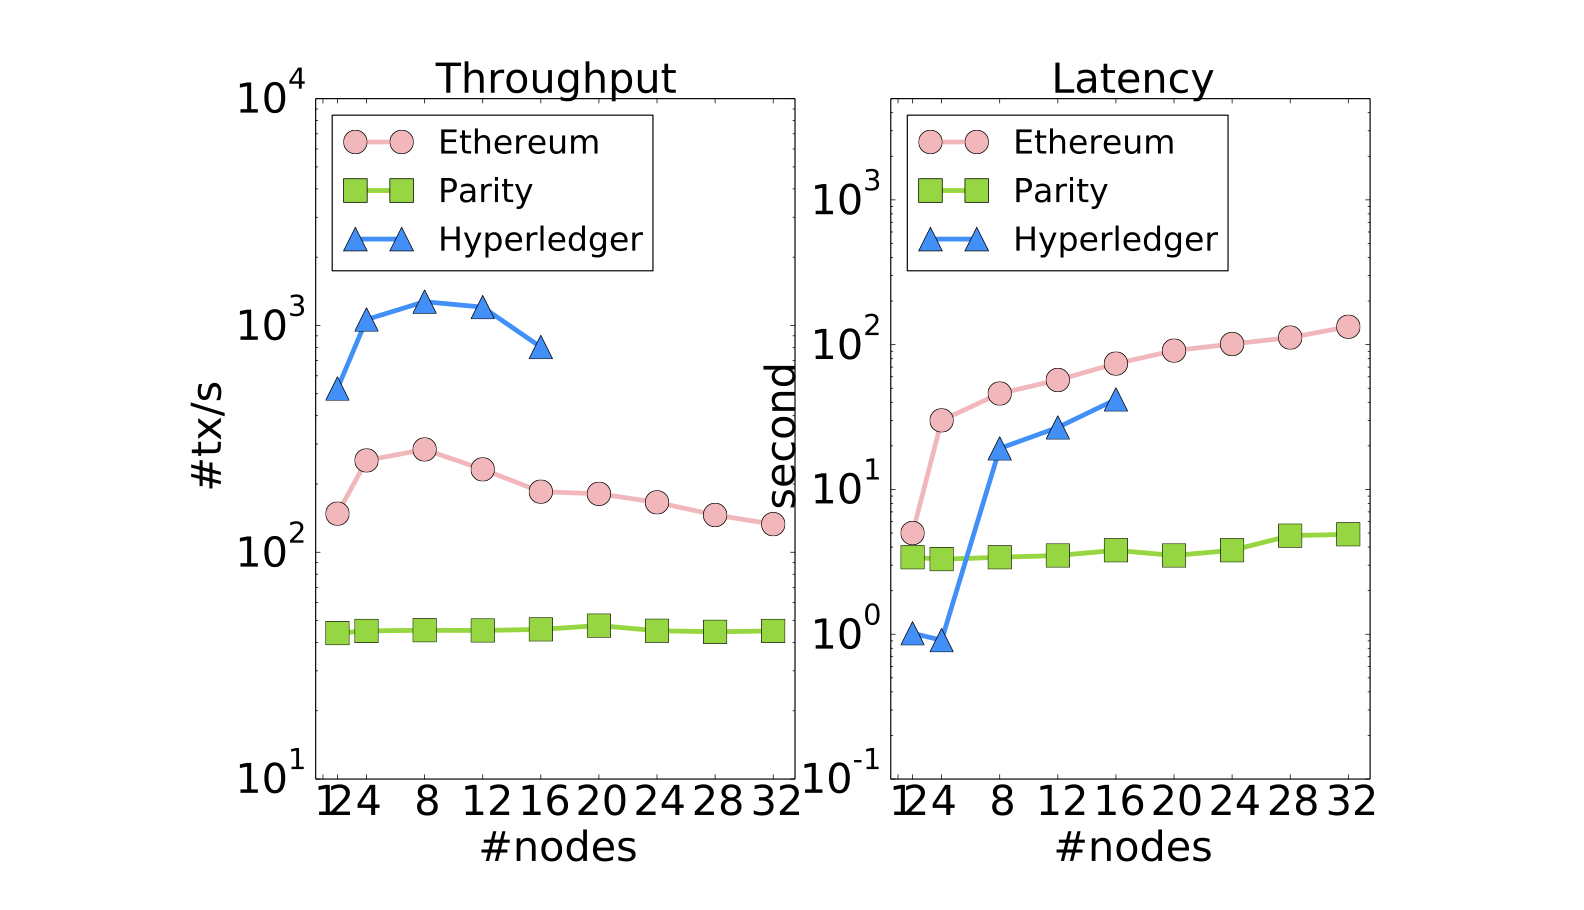
\includegraphics[width=15cm]{3-desafios-de-escalabilidade/figures/escalabilidade-perfomance1.png}}
                \caption{Performance scalability (with the same number of clients and servers). \cite{blockbench}, .}
                \label{perfomance-scability}
            \end{figure}

Agora, procederemos à análise do motivo pelo qual o sistema Hyperledger não conseguiu escalar além de 16 servidores e 16 clientes. Ao examinar o registro do sistema Hyperledger, identificou-se que os nós estavam tentando chegar a um consenso em relação a novas visões que continham lotes de transações, porém estavam falhando continuamente nesse processo. O que ocorreu foi que os servidores estavam em visões divergentes, resultando no recebimento de mensagens conflitantes de mudança de visão provenientes do restante da rede. Em essência, esses conflitos surgiram devido à rejeição das mensagens de consenso por parte de outros pares, em virtude do congestionamento do canal de mensagens. À medida que as mensagens eram descartadas, as visões divergiam progressivamente, culminando em um impasse no consenso.

Adicionalmente, observou-se que, ao longo do tempo, as solicitações dos clientes passaram a demandar mais tempo para serem concluídas, o que evidencia que os servidores estavam sobrecarregados no processamento das mensagens da rede. Contudo, é importante salientar que o protocolo original de PBFT garante tanto a vitalidade quanto a segurança. Portanto, a incapacidade do Hyperledger de escalar além de 16 servidores pode ser atribuída à implementação específica do protocolo.

Até o momento, os resultados obtidos indicam que a tentativa de escalonar tanto o número de clientes quanto o número de servidores resulta na degradação do desempenho, levando inclusive à falha do sistema Hyperledger nesse contexto.

A figura \ref{perfomance-scability2} ilustra uma observação relevante sobre o desempenho dos sistemas em análise. Conforme o número de servidores é incrementado, nota-se uma degradação no desempenho, indicando que os sistemas enfrentam sobrecargas na rede. Essa observação é particularmente pertinente devido à natureza dos sistemas em análise.

O Hyperledger, por sua característica de limitação da comunicação, apresenta um comportamento no qual o aumento do número de servidores resulta em uma intensificação da troca de mensagens e consequentemente uma maior sobrecarga. Por outro lado, o Ethereum, embora limitado pela capacidade de processamento, ainda demanda uma quantidade modesta de recursos de rede para a disseminação de transações e blocos para outros nós. Vale ressaltar que, em redes mais extensas, a dificuldade da rede é aumentada para acomodar os atrasos na propagação.

Uma constatação importante é que, para evitar divergências na rede, o nível de dificuldade é ajustado a uma taxa superior ao crescimento no número de nós. Portanto, uma das causas da degradação na taxa de transferência do Ethereum reside no tamanho da rede. Além disso, na configuração adotada, onde 8 clientes enviam solicitações exclusivamente para 8 servidores, nota-se que esses servidores nem sempre compartilham as transações entre si, mantendo a mineração de maneira independente em suas respectivas pools de transações. Isso resulta em uma subutilização da capacidade de mineração da rede.

Esse fenômeno revela a complexidade subjacente ao desempenho de sistemas de blockchain em ambientes com diferentes tamanhos de rede, bem como destaca a necessidade de abordagens específicas para otimizar a eficiência das operações em tais contextos. Essa análise oferece uma compreensão mais aprofundada dos desafios associados à escalabilidade e otimização de sistemas de blockchain em ambientes dinâmicos e diversificados.


            \begin{figure}[H]
                \centering
                \frame{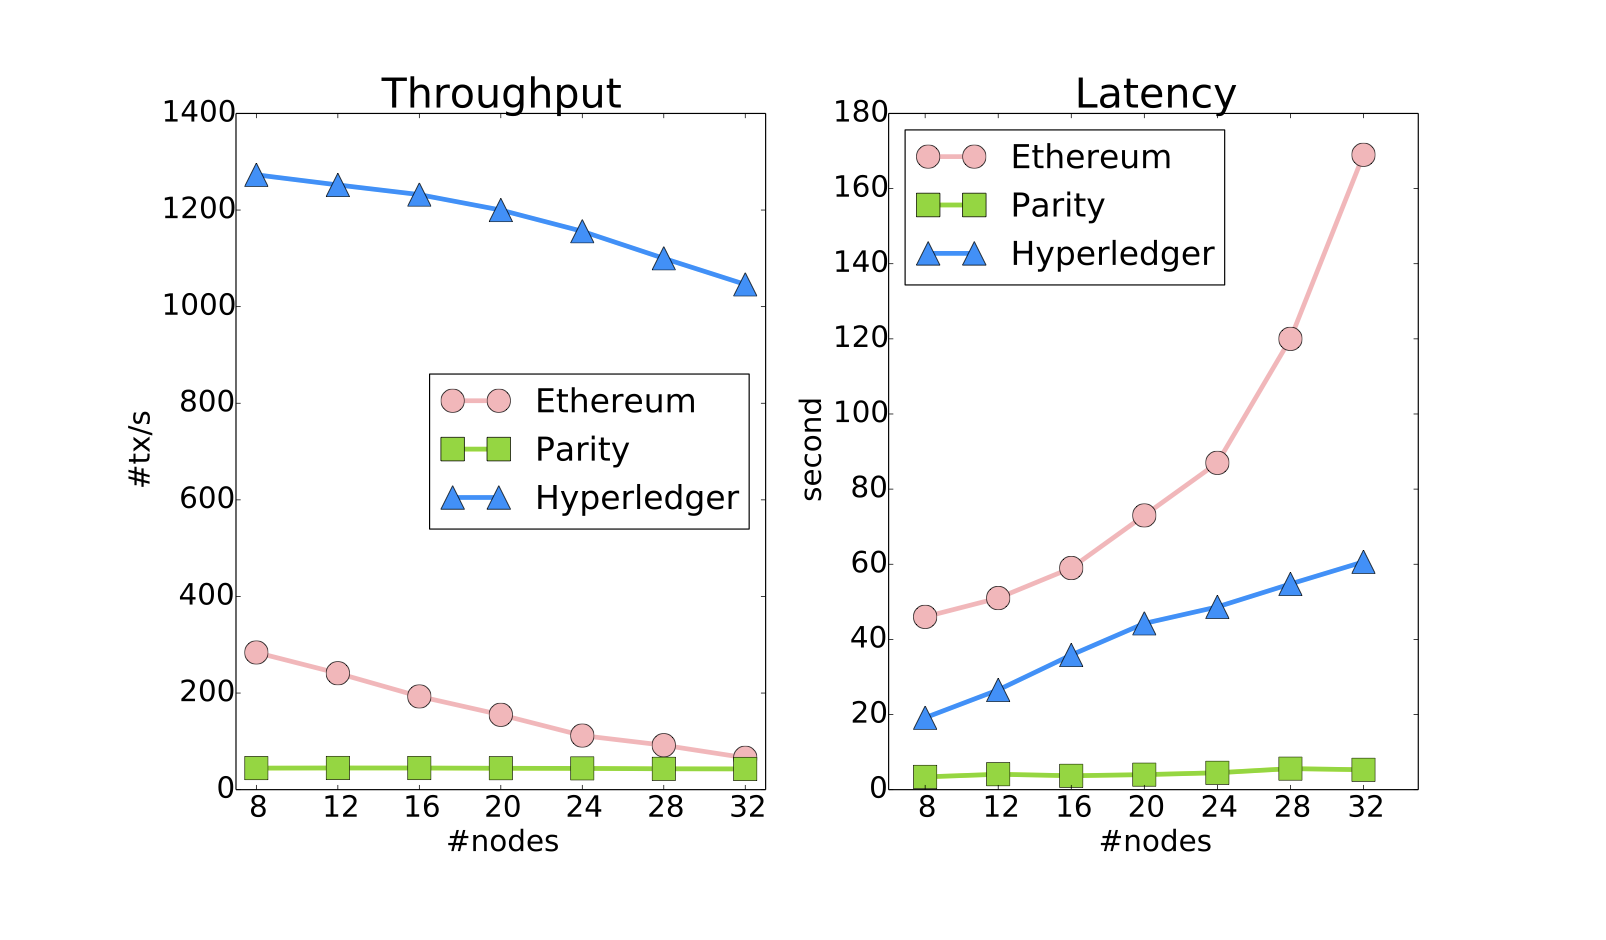
\includegraphics[width=15cm]{3-desafios-de-escalabilidade/figures/escalabilidade2.png}}
                \caption{Performance scalability (with 8 clients)). \cite{blockbench}, .}
                \label{perfomance-scability2}
            \end{figure}